\section{Sample Time}
A bottleneck on the accuracy of the final image is the amount of error introduced by the necessary sampling of the time-optimal velocity profile. There is a limit on the accuracy of a system that uses integration in order to achieve an outcome, as the smallest amount of error will magnify until the result is quite different from that which is desired. Since a digital processing device can only direct an integrating process at a limited rate, sampling errors will accumulate over time and cause the image to become inaccurate. Since upon initialisation of a trajectory the measured placement of the curves initial position resets the integration error, the error can only accumulate over a single curve. The effect of operating at differing sample frequencies can be seen in Figure \ref{fig:timestep}.

\begin{figure}[htbp]  
\includegraphics[width=\textwidth]{figures/performance/timestep.png}
\caption[Comparison of differing velocity sampling frequencies]{A comparison of velocity sampling frequencies. From top left to bottom right; 1) 50hz 2) 25Hz 3) 12.5Hz 4) 8.3Hz 5) 6.6Hz 6) 5Hz
\label{fig:timestep}}
\end{figure}  

Two effects are at play in the alteration of the sampling frequency. A limit exists on the increase of the sampling frequency beyond the frequency of the controller to undergo one iteration of the control loop. Beyond this point, above roughly 25Hz for the DoodleBot, commands begin to get skipped or are not active for a long enough duration to have an effect. This causes the type of distortion in the final image that can be seen in the top left profile in Figure \ref{fig:timestep}. The second effect on the accuracy of the output image is that of an increase in the sampling time corresponding to a looser approximation of the correct velocity profile. The looser an approximation becomes, the greater the integral error will become over the length of the curve. Figure \ref{fig:timestep} demonstrates this in the lower sampling frequencies. As the sampling frequency decreases the amount of error becomes progressively greater. Figure \ref{fig:tStep} demonstrates that the level of error in the final image is linearly correlated with respect to the sampling period and hence inversely proportional to the sampling frequency. 
\begin{figure}[htbp]  
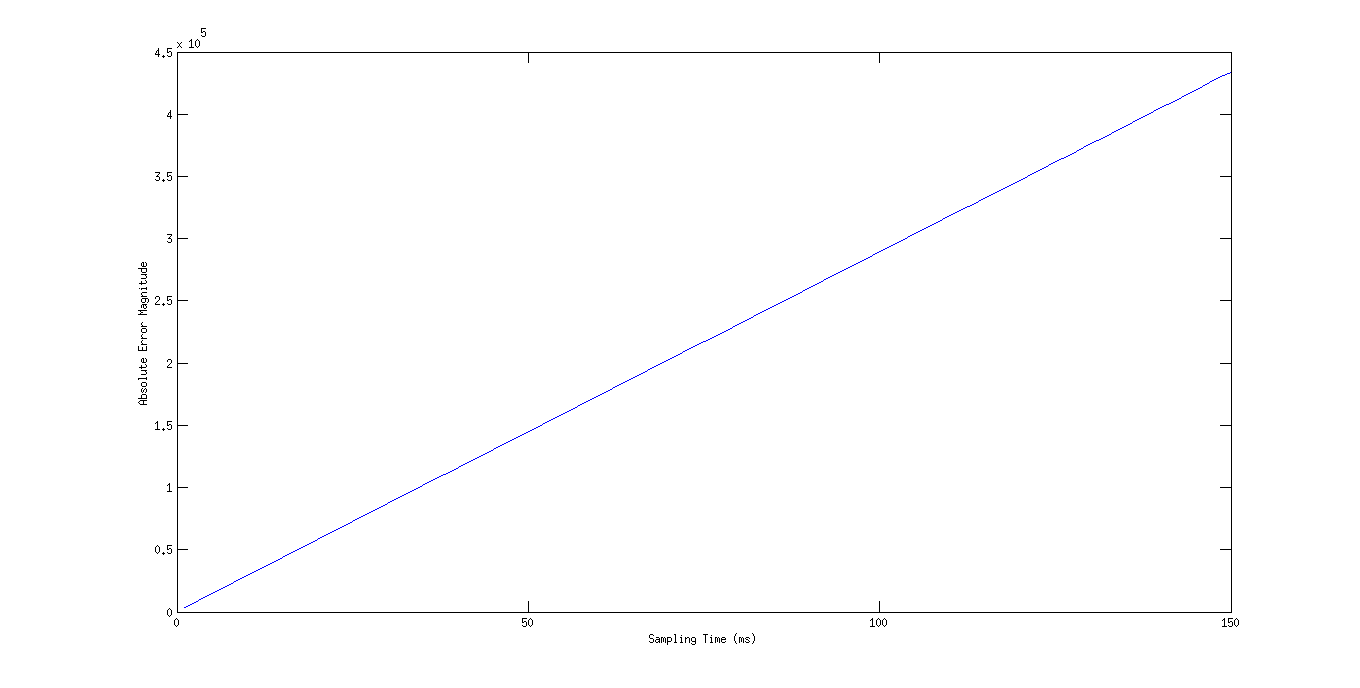
\includegraphics[width=\textwidth]{figures/performance/tStep.png}
\caption[Plot of error magnitude against velocity sampling period]{Error magnitude against velocity sampling period
\label{fig:tStep}}
\end{figure}  
It is evident that the best policy is to decrease the sample time until just before the limits of the control loop manifest. The DoodleBot was found to perform best at 25Hz, or with a 40ms sampling period.